\section{PLM}

\begin{frame}{PLM}
    \begin{figure}
        \resizebox{0.7 \textwidth}{!}{
            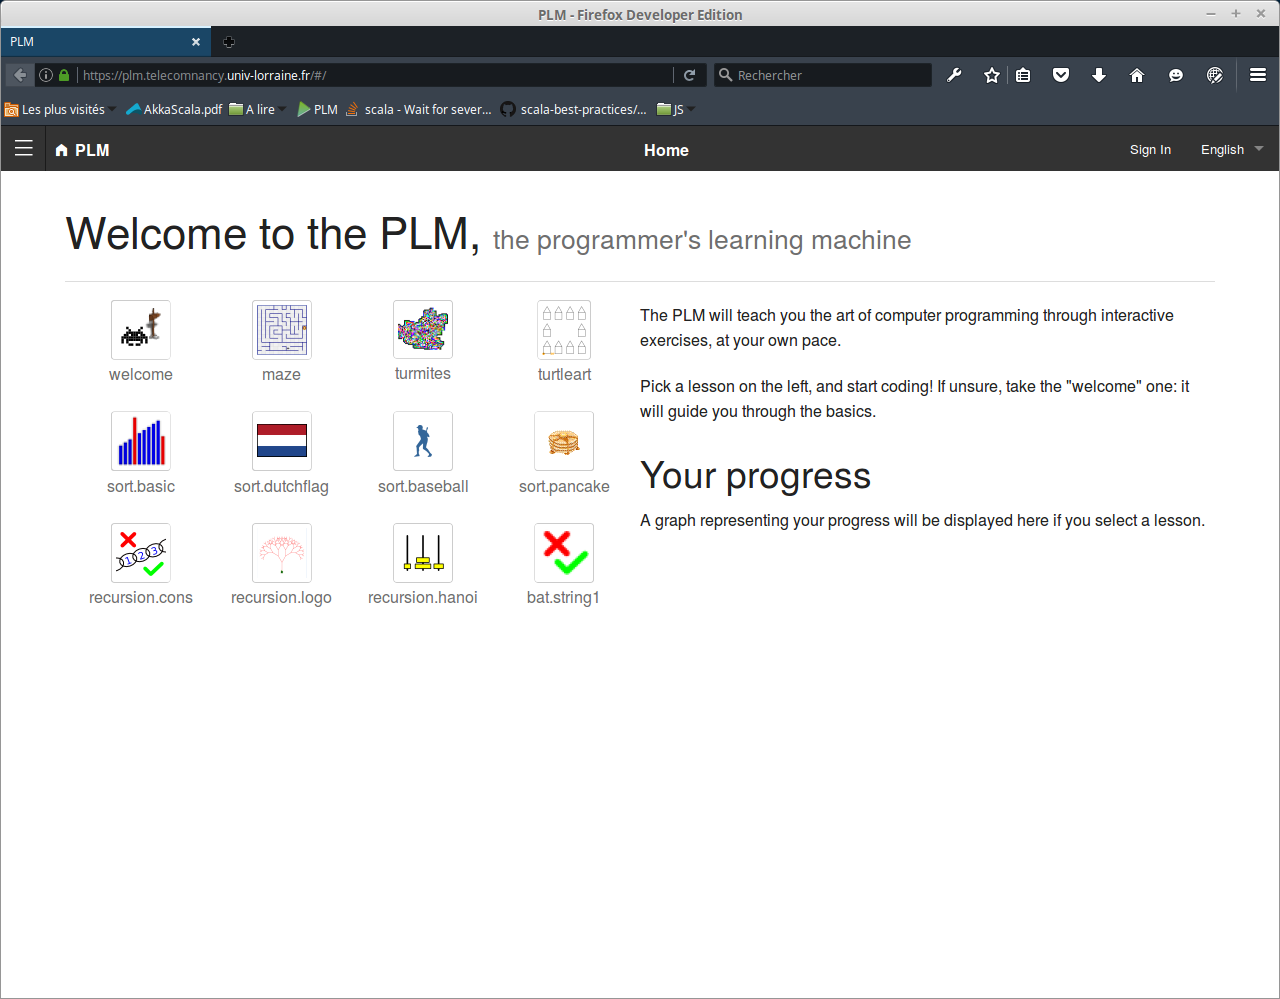
\includegraphics{img/screen-webPLM-1.png}
        }
    \end{figure}
    \vspace{-0.5cm}
    \begin{itemize}
        \item Application d'apprentissage de l'algorithmie et programmation
        \item Conçue pour un usage principalement autonome...
        \item ... avec enseignant(s) pour dépanner au besoin
    \end{itemize}
\end{frame}

\begin{frame}{Principe}
    \begin{figure}
        \resizebox{0.7 \textwidth}{!}{
            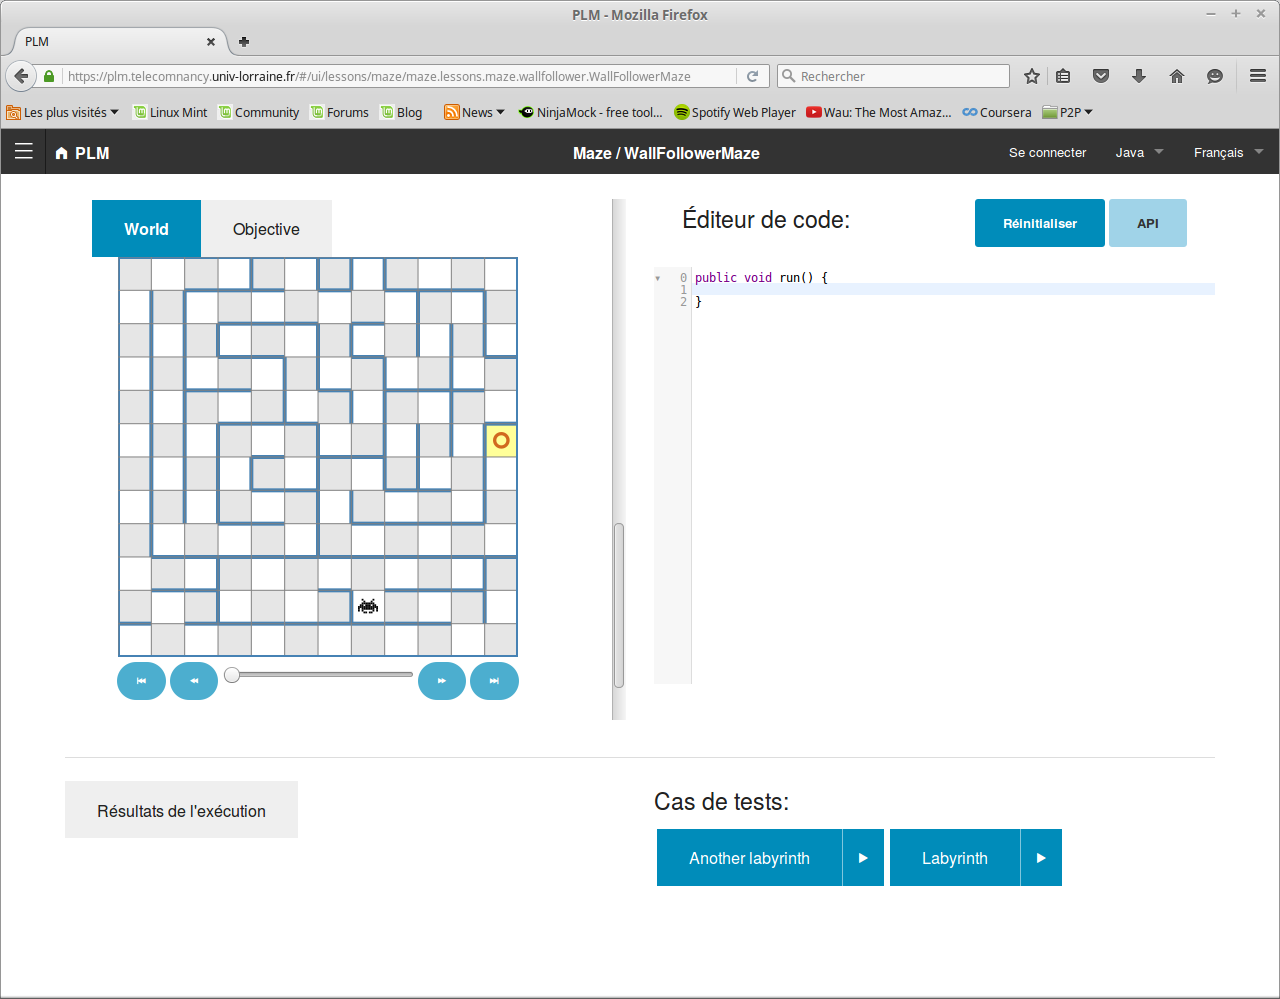
\includegraphics{img/maze.png}
        }
    \end{figure}
    \vspace{-0.5cm}
    \begin{itemize}
        \item Propose ensemble d'exercices, des bases de la programmation à la récursivité
        \item Étudiant-e peut soumettre un programme et visualiser ses effets
    \end{itemize}
\end{frame}

\begin{frame}{Contributions}
    \metroset{block=transparent}
    \begin{block}{Suivi de la progression des étudiant-es}
        \begin{itemize}
            \item Utilise git pour versionner le code soumis par l'étudiant-e
            \item Initialement, avait des pertes de données
            \item Correction et refactoring du code
        \end{itemize}
    \end{block}

    \begin{block}{Tests automatiques}
        \begin{itemize}
            \item Implémentation de tests d'intégration sur les parties critiques : \emph{git, solutions des exercices, instanciation des leçons}
            \item Mise en place d'un processus d'intégration continue
        \end{itemize}
    \end{block}
\end{frame}

\begin{frame}{Contributions - suite}
    \metroset{block=transparent}
    \begin{block}{Webification}
        \begin{itemize}
            \item Refactoring de l'architecture logicielle : suppression du singleton principal
            \item Séparation de l'exécution du code des apprenants en un composant dédié et isolé : \emph{plm-judge}
            \item Mise en place d'une architecture système passant à l'échelle
        \end{itemize}
    \end{block}
\end{frame}

\begin{frame}{Architecture système de PLM}
    \begin{figure}
        \resizebox{\textwidth}{!}{
            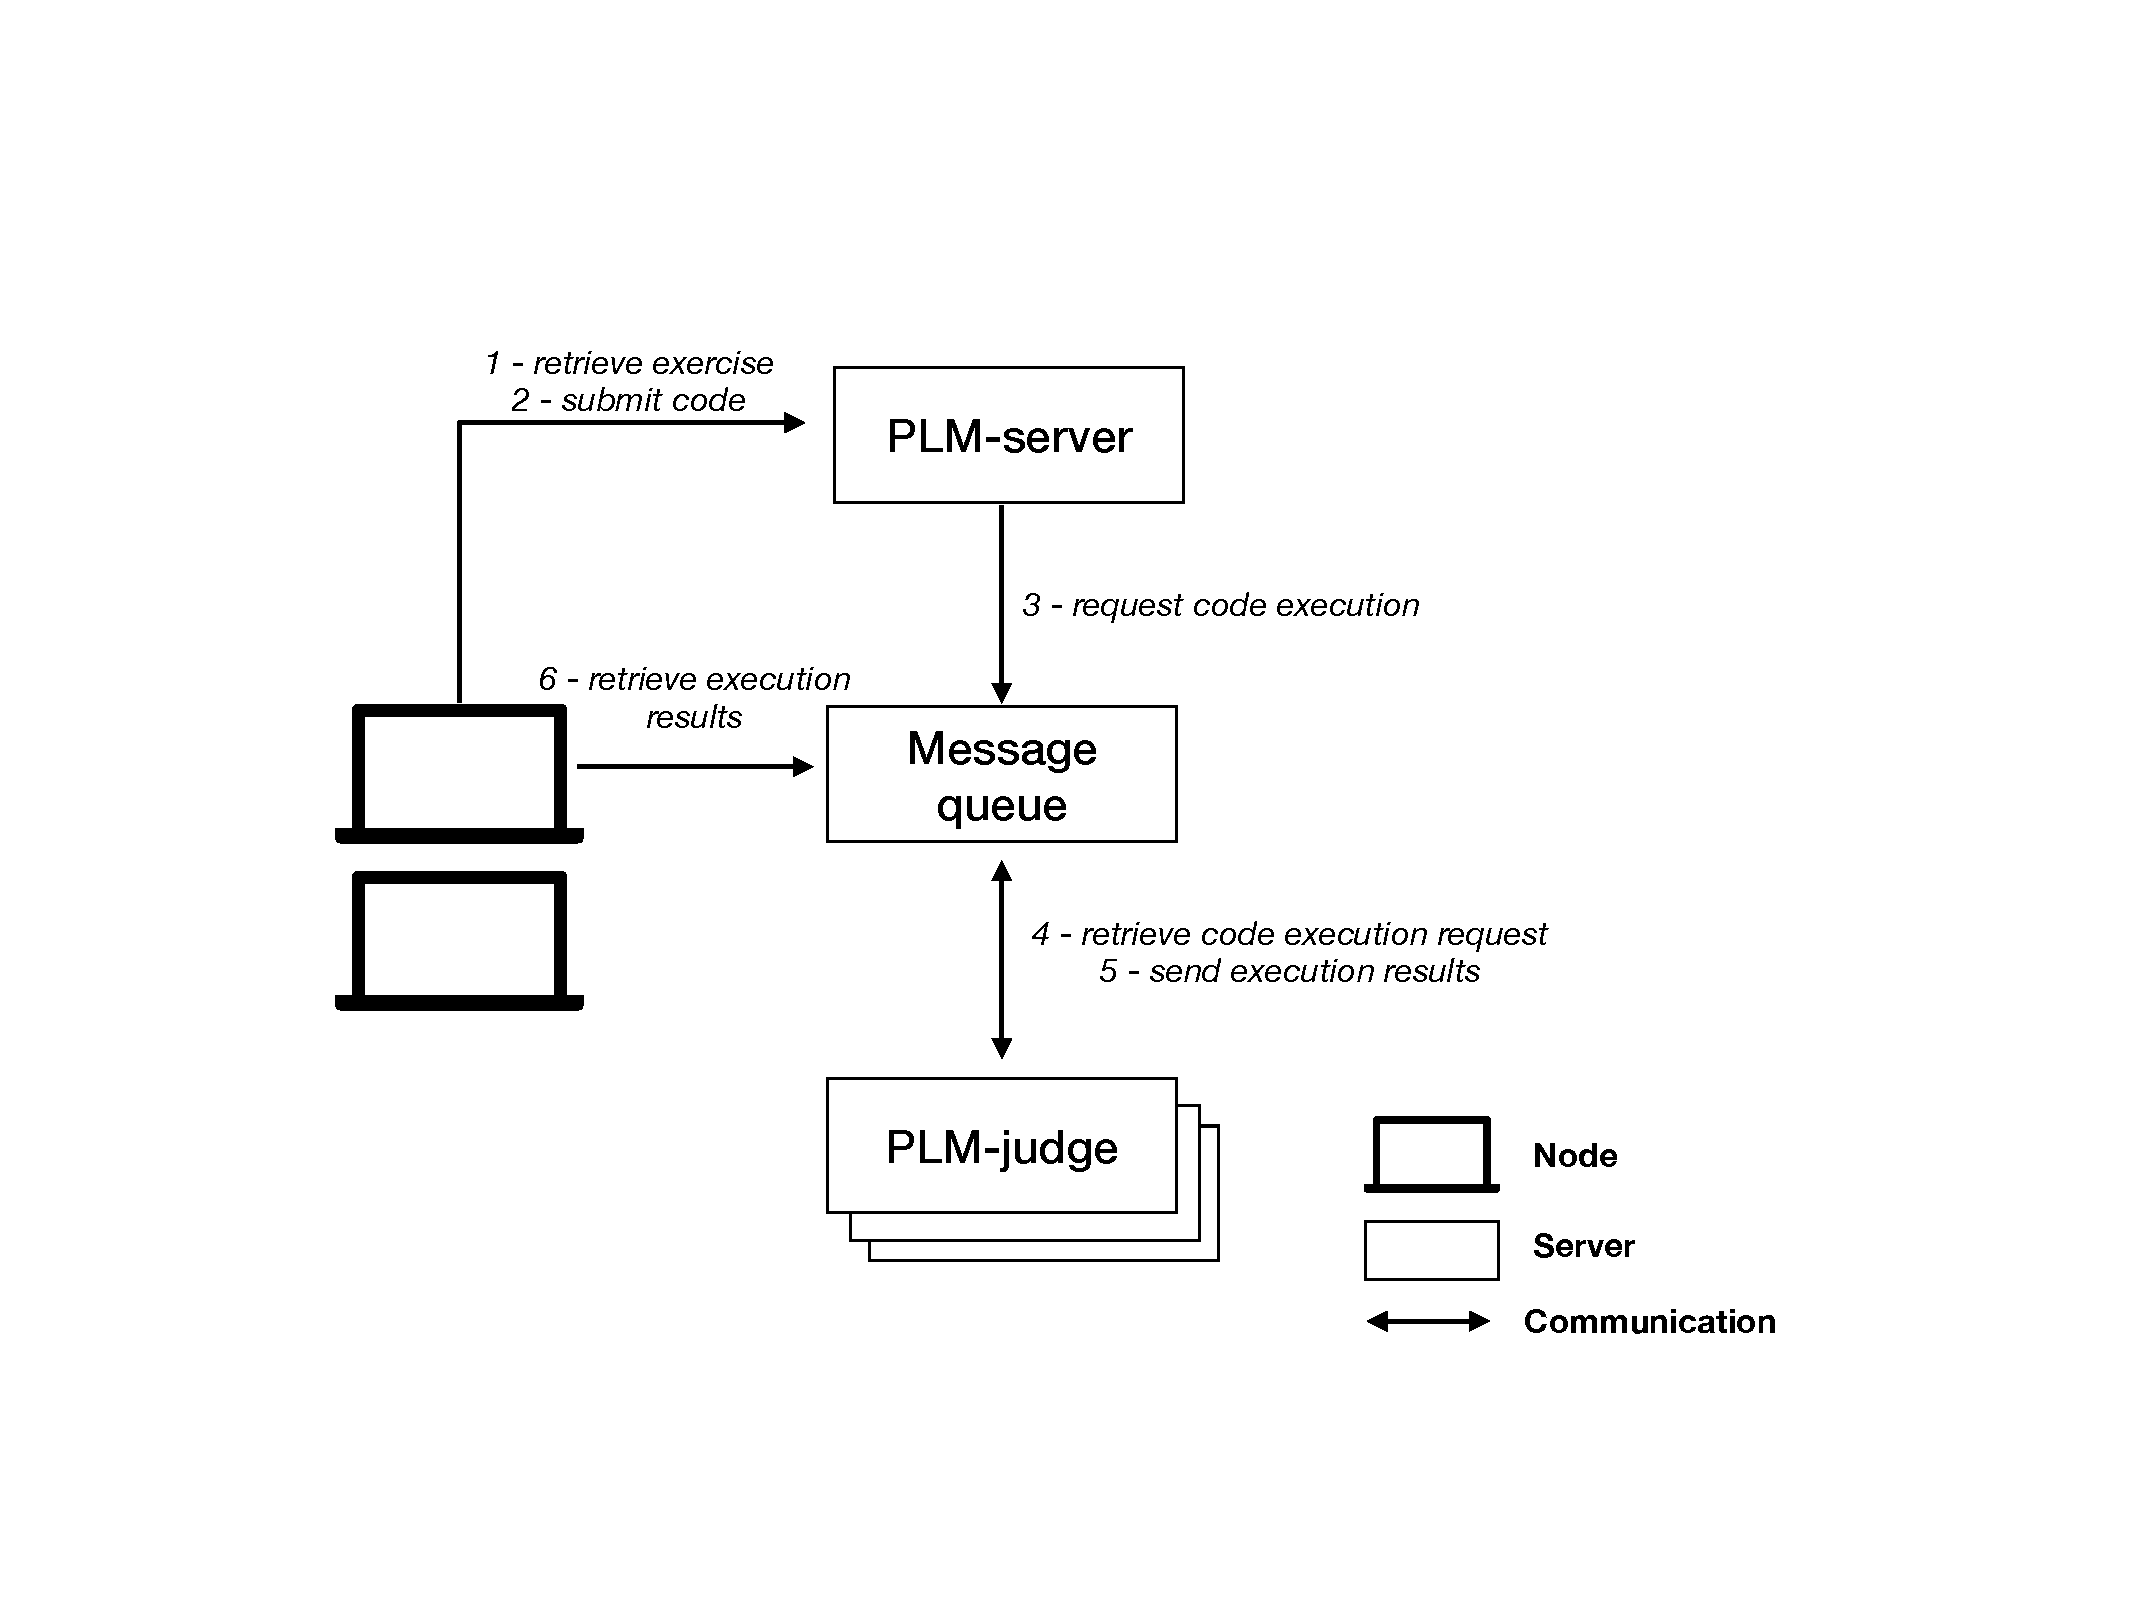
\includegraphics[page=1, trim=4cm 3cm 3cm 4cm, clip, width=.7\linewidth]{img/plm-figures.pdf}
            }
    \end{figure}
\end{frame}
